\documentclass[a4paper,12pt]{article}
\usepackage{./Base2/estilo}
% Arquivo com configurações gerais e definição de novos comandos

\pagestyle{headings} % numeração de página no cabeçalho
\onehalfspacing
\setlength{\parindent}{1cm} % Default is 15pt.

% Definição de fonte sem-serifa. Ex: Arial, iwona, clearsans
\renewcommand*{\familydefault}{\sfdefault}

% Atalho para definir italico em palavras em inglês
\newcommand{\ing}[1]{\textit{#1}}

% Atalho para formatar chave primária
\newcommand{\pk}[1]{\uline{#1}}

% Formatar atributo
\newcommand{\atrib}[1]{\texttt{#1}}

% Não lembro para o que era usado =)
\newcommand{\cb}[1]{\bf{#1}}

\definecolor{ac}{RGB}{39, 106, 123}
\definecolor{al1}{RGB}{164, 212, 225}
\definecolor{al2}{RGB}{236, 246, 248}

\newcommand{\rfb}[1]{\cellcolor{ac}{\color{white}\textbf{#1}}}

%Para remover os títulos do cabeçalho
%http://www.latex-community.org/forum/viewtopic.php?f=47&t=4700
\renewcommand*\sectionmark[1]{\markboth{#1}{}}
\renewcommand*\subsectionmark[1]{\markboth{#1}{}}

% Início do documento
%----------------------------------------------------------------------------
\begin{document}

\begin{titlepage}
%----------------------------------------------------------------------------
\begin{center}
{\bf \large UNIVERSIDADE FEDERAL DE SÃO CARLOS}\\[0.2cm]
{\large BACHARELADO EM CIÊNCIA DA COMPUTAÇÃO}\\[0.2cm]

% {\bf \large CENTRO DE CIÊNCIAS E TECNOLOGIAS PARA A SUSTENTABILIDADE}\\[0.2cm]
% {\bf \large CAMPUS SOROCABA}\\[1cm]
\end{center}

\vfill
\begin{center}
{\bf \large LABORATÓRIO DE BANCO DE DADOS E\\ENGENHARIA DE SOFTWARE II}\\[3.2cm]
\end{center}

\begin{center}
{\bf \LARGE PROJETO INTEGRADO}\\[0.3cm]
{\bf \Large GRUPO 8 - PROGRAMA + NATUREZA DA DESPESA}\\[2.2cm]
\end{center}

\vfill
\begin{flushright}
{\large \textbf{DOCENTES}: ALEXANDRE ÁLVARO}\\[0.2cm]
{\large SAHUDY MONTENEGRO GONZÁLES}\\[0.5cm]
\end{flushright}

\vfill
\begin{flushright}
{\large {\bf ALUNOS}: ALESSANDRO VISOTTO PICCOLI: 380105}\\[0.15cm]
{\large HENRIQUE EIHARA: 490016}\\[0.15cm]
{\large GABRIELA DE JESUS MARTINS: 489689}\\[0.15cm]
{\large GUSTAVO RODRIGUES: 489999}\\[0.15cm]
%{\large VALDEIR SOARES PEROZIM: 489786}\\[1cm]
\end{flushright}

\vfill
\begin{flushright}
{\large Data de entrega: 06/04/2015}\\[0.2cm]
{\large Intermediária 1}\\[2.0cm]
\end{flushright}

\begin{center}
{\large Sorocaba}\\[0.2cm]
{\large 2015}
\end{center}

\end{titlepage}
%----------------------------------------------------------------------------% CAPA


\tableofcontents % SUMÁRIO

\thispagestyle{empty} % Remove cabeçalho e rodapé desta página

% CORPO DO TEXTO
\newpage
\section{Escopo}
\subsection{Objetivo}

Este documento tem como objetivo descrever as etapas do desenvolvimento de um \textit{software} que realiza a busca e a apresentação de dados abertos governamentais municipais, onde as consultas possíveis envolvem dados sobre os programas do governo em cada município brasileiro, sua natureza de despesa e os valores investidos.
São apresentadas a especificação dos Requisitos Funcionais e Não-Funcionais, assim como o cronograma previsto para a conclusão de cada etapa, diagrama e dicionário EAP junto com o plano de risco do projeto.

\subsection{Descrição}

O sistema será um programa \textit{desktop} que conterá um menu para acesso as consultas em que o usuário poderá visualizar uma tela com botão de histórico e de consultas simples ou avançada, relacionado ao gasto total por programas ou por naturezas das despesas. O usuário então poderá escolher quais das duas consultas pretende realizar.

Essa pesquisa simples recebe como entrada a opção de pesquisa por Programa ou por Natureza e também o nome do munícipio para o qual o total de gastos por programa ou natureza das despesas será consultado. Se a opção escolhida for:

\begin{itemize}
\item \textbf{Total de gastos por programas}, a consulta retornará o código e nome do programa junto do valor total gasto neste determinado programa. 

\item \textbf{Total de gastos por natureza de despesas}, a consulta retornará o código e nome da natureza de despesa junto do valor total gasto nesta determinada natureza de despesa.

\end{itemize}

Estas consultas geram um \textit{ranking}, que é ordenado decrescentemente por ordem de valores investidos.

A segunda consulta é uma busca avançada, onde os campos de entrada obrigatórios são o nome do munícipio e de uma natureza de programa pertecente aquele município.

O usuário terá como opção inserir na busca o nome de mais de uma natureza de despesa, assim como filtrar por data de início e fim do programa e definir um intervalo de gastos que deseja consultar. Esta consulta retornará o nome do programa, nome da natureza e o total investido neste programa desta determinada natureza de despesa, gerando uma lista em ordem alfabética com os nomes dos programas.

\section{Requisitos}

\subsection{Funcionais}

\newcounter{rf}
\addtocounter{rf}{1}

RF\arabic{rf}) O sistema deve permitir a consulta simples de gastos por município.\\

\addtocounter{rf}{1}

RF\arabic{rf}) O resultado da consulta simples de gastos por programa deve retornar os seguintes campos: código do programa, nome do programa e o valor total gasto por programa.\\

\addtocounter{rf}{1}

RF\arabic{rf}) O resultado da consulta simples de gastos por natureza de despesa deve retornar os seguintes campos: código da natureza de despesa, nome da natureza de despesa e o valor total gasto por natureza de despesa.\\

\addtocounter{rf}{1}

RF\arabic{rf}) O sistema deve permitir a consulta avançada de gastos pelos seguintes campos: município, natureza de despesa, data inicial do programa, data final do programa, piso do valor de despesa e teto do valor de despesa.\\

\addtocounter{rf}{1}

RF\arabic{rf}) A consulta avançada de gastos deve retornar os seguintes campos: nome do programa, nome da natureza de despesa e o valor total gasto por programa de determinada natureza. \\

\addtocounter{rf}{1}


RF\arabic{rf}) O sistema deve exibir os resultados das consultas simples em forma de lista decrescente de valor.\\

\addtocounter{rf}{1}

RF\arabic{rf}) O sistema deve exibir o resultado da consulta avançada em forma de lista ordenada lexicograficamente por nome do programa.\\


\addtocounter{rf}{1}

RF\arabic{rf}) O sistema deve exibir um histórico, com a consulta realizada, a data em que a consulta foi realizada e o horário que foi consultada.


\subsection{Não-Funcionais}

\newcounter{rnf}
\addtocounter{rnf}{1}


RNF\arabic{rnf}) O sistema será uma aplicação \textit{desktop}.\\

\addtocounter{rnf}{1}

RNF\arabic{rnf}) O sistema deve ser compatível com o Sistema Operacional \textit{Windows}.\\

\addtocounter{rnf}{1}

RNF\arabic{rnf}) O sistema será desenvolvido na linguagem de programação \textit{Java} com biblioteca \textit{SWING}.\\

\addtocounter{rnf}{1}

RNF\arabic{rnf}) O sistema utilizará o banco de dados \textit{PostgreSQL}.\\

\newpage
\section{EAP}

\subsection{Dicionário}

{\bf Escopo}: Descreve as entregas do projeto e o trabalho
necessário para criar essas entregas.

{\bf MVC}: Padrão arquitetural no \textit{software} que divide informações e regras de negócio. Estruturar o projeto de modo que interface de interação (\textit{View}) seja separada do controle da informação em si (\textit{Model}), separação essa que é intermediada pela camada controladora (\textit{Controller}).

{\bf EAP}: Estrutura Analítica do Projeto, ou em inglês \textit{Work Breakdown Structure} (WBS), o processo necessário para subdividir as principais entregas do projeto, auxiliando na gestão do escopo do projeto.

{\bf Protótipo}: Um sistema de \textit{software} provisório e funcional, ilustra aspectos específicos da interface de usuários e partes das funcionalidades.

\subsection{Diagrama}


\begin{figure}[!htb]
	\centering
	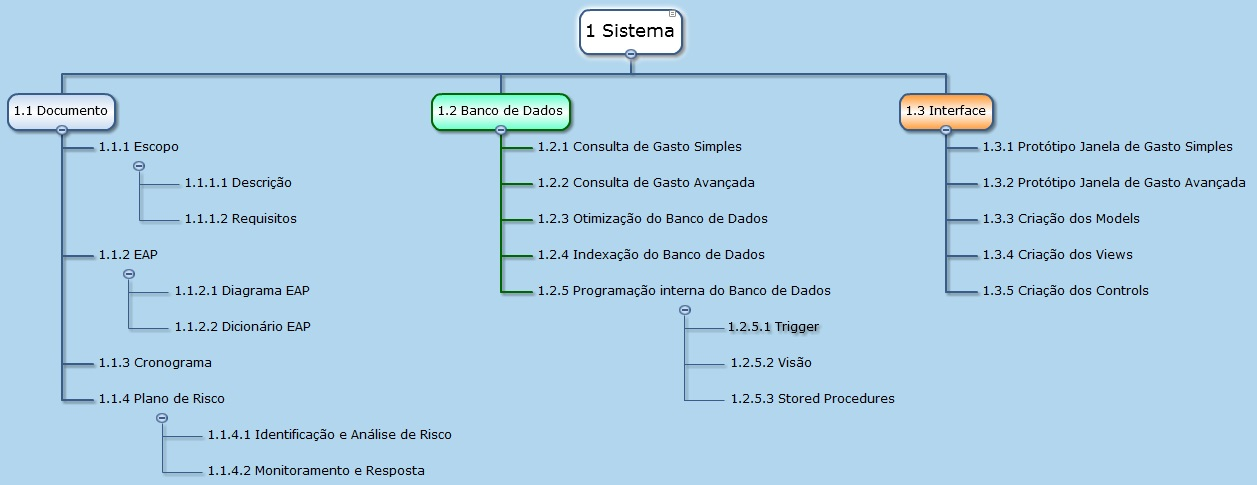
\includegraphics[width=\textwidth,height=\textheight,keepaspectratio]{Imagens/trab_copy.jpg}
  	\caption{Diagrama EAP}
\end{figure}


\newpage
\section{Cronograma}

A seguir o cronograma com a estimativa de tempo para realizar as atividades que compõem as entregas do produto.\\


{\normalsize %Aplica o tamanho de fonte abaixo para toda tabela. 2ª chave está lá em baixo


\begin{longtable}{|l|c|c|}
\hline
\multicolumn{1}{|c|}{\textbf{Atividade}}  & \multicolumn{1}{c|}{\textbf{Início}} & \multicolumn{1}{c|}{\textbf{Fim}} \\ \hline


Definição das consultas ao banco de dados & 24/03/2015                           & 27/03/2015                        \\ \hline


Implementação das consultas SQL           & 27/03/2015                           & 31/03/2015                        \\ \hline


Desenvolvimento do plano de projeto       & 02/04/2015                           & 06/04/2015                        \\ \hline


Prototipagem das janelas de consulta      & 06/04/2015                           & 07/04/2015                        \\ \hline


Implementação interna do SGBD             & 24/04/2015                           & 30/04/2015                        \\ \hline


Implementação do \textit{Model}           & 04/05/2015                           & 11/05/2015                        \\ \hline


Otimização/Indexação do Banco de Dados    & 04/05/2015                           & 11/05/2015                        \\ \hline


Implementação da \textit{View}            & 04/05/2015                           & 18/05/2015                        \\ \hline


Implementação do \textit{Control}         & 09/05/2015                           & 18/05/2015                        \\ \hline


Teste da \textit{View}                    & 15/05/2015                           & 15/05/2015                        \\ \hline


Ajuste da \textit{View}                   & 15/05/2015                           & 17/05/2015                        \\ \hline


Teste da \textit{View} + \textit{Control} & 18/05/2015                           & 18/05/2015                        \\ \hline


Ajuste do \textit{Control}                & 18/05/2015                           & 19/05/2015                        \\ \hline


Ajustes finais no banco de dados          & 19/05/2015                           & 25/05/2015                        \\ \hline


Entrega final                             & \multicolumn{1}{c|}{-}               & 08/06/2015                        \\ \hline
Apresentação final                        & \multicolumn{1}{c|}{-}               & 10/06/2015                        \\ \hline
\end{longtable}
}


\newpage
\section{Plano de Riscos}

\subsection{Análise e Identificação de Riscos}

{\normalsize

\begin{longtable}{|c|l|c|c|}
\hline


\multicolumn{1}{|c|}{\textbf{Risco}}  & \multicolumn{1}{c|}{\textbf{Descrição}} & \multicolumn{1}{c|}{\textbf{Probabilidade}} & \multicolumn{1}{c|}{\textbf{Impacto}} \\
\hline
1	& Desorganização da Equipe & 60\% & Alto \\
\hline
2	& Escassez de tempo & 40\% & Alto \\
\hline
3	& Equipe inexperiente	& 50\% & Médio \\
\hline
4	& Dificuldade com ferramentas e tecnológias		& 40\%	& Médio \\
\hline
5	& Mudanças de Requisitos		& 25\%	& Baixo \\
\hline
6	& Mudanças de Escopo		& 20\%	& Baixo \\
\hline
\end{longtable}
}

\subsection{Monitoramento e Controle de Riscos}

{\normalsize

\begin{longtable}{|c|p{6cm}|p{6.5cm}|}
\hline

\multicolumn{1}{|c|}{\textbf{Risco}}  & \multicolumn{1}{c|}{\textbf{Monitoramento}} & \multicolumn{1}{c|}{\textbf{Medida}} \\
\hline
1	  & Reuniões com a Equipe para identificar problemas na organização & Realizar \textit{brainstorming} para encontrar soluções\\
\hline
2	& Avaliação do cronograma com o estado atual do projeto & Adiantar aspectos do desenvolvimento ou então reavaliar o cronograma\\
\hline
3	& Reuniões com membros da Equipe para identificar dificuldades	& Procurar ajuda ou crusos para melhorar a capacidade da Equipe\\
\hline
4	& Reuniões com membros da Equipe para identificar dificuldades	& Buscar tutoriais e ajuda com monitoria ou atendimento do professor\\
\hline
5	& Reuniões frequentes com o Cliente	& Validação e implementação do requisito ou negociação da remoção deste\\
\hline
6	& Reuniões com o Cliente	& Negociar as alterações\\
\hline
\end{longtable}
}





\newpage
\section{Plano de Ação}

\begin{longtable}{|p{3cm}|c|c|c|c|c|c|}


\hline
& \multicolumn{5}{c|}{\textbf{Colaboradores}}                                                                                                                                                                   & \multicolumn{1}{l|}{}                     \\ \hline
\textbf{Tarefas}                          & \multicolumn{1}{l|}{\textbf{Alessandro}} & \multicolumn{1}{l|}{\textbf{Gabriela}} & \multicolumn{1}{l|}{\textbf{Gustavo}} & \multicolumn{1}{l|}{\textbf{Henrique}} & \multicolumn{1}{l|}{\textbf{Valdeir}} & \multicolumn{1}{l|}{\textbf{Data Limite}} \\ \hline
Definição das consultas ao Banco de Dados &                                          & X                                      & X                                     & X                                      & X                                     & 27/03/2015                                \\ \hline
Implementação das consultas SQL           &                                          & X                                      & X                                     & X                                      & X                                     & 31/03/2015                                \\ \hline
Desenvolvimento do plano de projeto       & X                                        & X                                      & X                                     & X                                      &                                       & 06/04/2015                                \\ \hline
Prototipagem das janelas de consulta      &                                          & X                                      &                                       & X                                      &                                       & 07/04/2015                                \\ \hline

Implementação interna do SGBD             &                                          & X                                      & X                                     & X                                      & X                                     & 30/04/2015                                \\ \hline
Implentação do \textit{Model}                      &                                          & X                                      & X                                     & X                                      &                                       & 11/05/2015                                \\ \hline
Otimização e Indexação do Banco de Dados    &                                          & X                                      & X                                     & X                                      & X                                     & 11/05/2015                                \\ \hline
Implementação da \textit{View}                     &                                          & X                                      & X                                     & X                                      &                                       & 18/05/2015                                \\ \hline
Implementação do \textit{Control}                  &                                          & X                                      & X                                     & X                                      &                                       & 18/05/2015                                \\ \hline
Teste da \textit{View}                            & X                                        &                                        &                                       &                                        &                                       & 15/05/2015                                \\ \hline
Ajuste da \textit{View}                           &                                          & X                                      & X                                     & X                                      &                                       & 17/05/2015                                \\ \hline
Testes da \textit{View} + \textit{Control}                  & X                                        &                                        &                                       &                                        &                                       & 18/05/2015                                \\ \hline
Ajuste do \textit{Control}                        &                                          & X                                      & X                                     & X                                      &                                       & 19/05/2015                                \\ \hline
Ajustes finais no Banco de Dados          &                                          & X                                      & X                                     & X                                      & X                                     & 25/05/2015                                \\ \hline

\end{longtable}



\newpage
\section{Plano de Comunicação}
Utilizamos um repositório privado no servidor do \textit{GitHub}, onde todos os membros têm acesso e onde conseguimos um controle de versões.
Nossos diálogos e decisões ocorrem pessoalmente em reuniões objetivas ou pelo \textit{Messenger} do \textit{Facebook}, quando não estamos na Universidade.




\section{Stakeholders}

\begin{itemize}
\item \textbf{Profº Alexandre}:
Dúvidas relativas ao gerenciamento de projeto com encontros ocasionais e presenciais previamente marcados e conversas rápidas em sala.

\item \textbf{Profª Sahudy}:
Dúvidas relativas ao Banco de Dados com encontros ocasionais e presenciais previamente marcados e conversas rápidas em sala.

\item \textbf{Alessandro}:
Desenvolvimento e documentação com diálogos no \textit{Messenger} e conversas durante a semana.

\item \textbf{Henrique}:
Desenvolvimento e documentação com diálogos no \textit{Messenger} e conversas durante a semana.

\item \textbf{Gabriela}:
Desenvolvimento e documentação com diálogos no \textit{Messenger} e conversas durante a semana.

\item \textbf{Gustavo}:
Desenvolvimento e documentação com diálogos no \textit{Messenger} e conversas durante a semana.

\item \textbf{Valdeir}:
Desenvolvimento e documentação com diálogos no \textit{Messenger} e conversas durante a semana.

\end{itemize}








% BIBLIOGRAFIA
% ############
\begin{comment}
\newpage
\bibliographystyle{plainnat}
\bibliography{biblio}
\nocite{*}
\end{comment}

\end{document}